\documentclass[a4paper, 11pt, oneside]{article}

% To use this template, you have to have a halfway complete LaTeX
% installation and you have to run pdflatex, followed by bibtex,
% following by one-two more pdflatex runs.
%
% Note thad usimg a spel chequer (e.g. ispell, aspell) is generolz
% a very guud ideo.

\usepackage[utf8]{inputenc}
\usepackage[a4paper, top=3cm, bottom=3cm, left=3cm, right=3cm]{geometry}
\renewcommand{\familydefault}{\sfdefault}
\usepackage{helvet}
\usepackage{listings}
\usepackage[english]{babel} %% typographie française
\usepackage[style=numeric, language=english]{biblatex}
\usepackage{parskip} %% blank lines between paragraphs, no indent
\usepackage[margin=1cm]{caption,subcaption}%% give long captions a margin
\usepackage{booktabs} %% typesetting nice tables
\usepackage[pdftex]{graphicx} %% include graphics, preferrably pdf
\usepackage[pdftex]{hyperref} %% many PDF options can be set here
\usepackage{amsmath}
\usepackage{amsthm}
\usepackage{csquotes}
\usepackage{minted}
\usepackage{tikz}
\usepackage{cleveref}
\pdfadjustspacing=1 %% force LaTeX-like character spacing

\newcommand{\mylastname}{Sirotkina}
\newcommand{\myfirstname}{Veronika}
\newcommand{\mynumber}{30006541}
\newcommand{\myname}{\myfirstname{} \mylastname{}}
\newcommand{\mytitle}{Local-first Collaboration on Relational Data}
\newcommand{\mysupervisor}{Anton Podkopaev}

\theoremstyle{definition}
\newtheorem{definition}{Definition}[section]

\hypersetup{
pdfauthor={\myname},
pdftitle={\mytitle},
pdfkeywords={},
colorlinks={true},
linkcolor={blue}
}

\addbibresource{refs.bib}

\begin{document}
\pagenumbering{roman}

\thispagestyle{empty}

\begin{flushright}

\includegraphics[scale=0.8]{img/bsc-logo.png}
\end{flushright}
\vspace*{40mm}
\begin{center}
\huge \textbf{\mytitle}
\end{center}
\vspace*{4mm}
\begin{center}
\Large by
\end{center}
\vspace*{4mm}
\begin{center}
\LARGE \textbf{\myname}
\end{center}
\vspace*{20mm}
\begin{center}
\Large Bachelor Thesis in Computer Science
\end{center}
\vfill
\begin{flushleft}
\large Submission: \today \hfill Supervisor: \mysupervisor \\ \rule{\textwidth}{1pt}
\end{flushleft}
\begin{center}
Constructor University $|$ School of Computer Science and Engineering
\end{center}

\newpage
\thispagestyle{empty}

\begin{center}
\Large \textbf{Statutory Declaration}
\vspace*{8mm}
\end{center}

\begin{center}
\begin{tabular}{|l|p{85mm}|}
\hline
Family Name, Given/First Name & \mylastname, \myfirstname \\
Matriculation number          & \mynumber                 \\
Kind of thesis submitted      & Bachelor Thesis           \\
\hline
\end{tabular}
\vspace*{8mm}
\end{center}

\subsection*{English: Declaration of Authorship}

I hereby declare that the thesis submitted was created and written solely by
myself without any external support. Any sources, direct or indirect, are marked
as such. I am aware of the fact that the contents of the thesis in digital
form may be revised with regard to usage of unauthorized aid as well as
whether the whole or parts of it may be identified as plagiarism. I do agree my
work to be entered into a database for it to be compared with existing sources,
where it will remain in order to enable further comparisons with future theses.
This does not grant any rights of reproduction and usage, however.

This document was neither presented to any other examination board nor has it
been published.

\subsection*{German: Erklärung der Autorenschaft (Urheberschaft)}

Ich erkläre hiermit, dass die vorliegende Arbeit ohne fremde Hilfe
ausschließlich von mir erstellt und geschrieben worden ist. Jedwede verwendeten
Quellen, direkter oder indirekter Art, sind als solche kenntlich gemacht worden.
Mir ist die Tatsache bewusst, dass der Inhalt der Thesis in digitaler Form geprüft
werden kann im Hinblick darauf, ob es sich ganz oder in Teilen um ein Plagiat
handelt. Ich bin damit einverstanden, dass meine Arbeit in einer Datenbank
eingegeben werden kann, um mit bereits bestehenden Quellen verglichen zu werden
und dort auch verbleibt, um mit zukünftigen Arbeiten verglichen werden zu
können. Dies berechtigt jedoch nicht zur Verwendung oder Vervielfältigung.

Diese Arbeit wurde noch keiner anderen Prüfungsbehörde vorgelegt noch wurde sie
bisher veröffentlicht.

\vspace{20mm}

\dotfill\\ Date, Signature

\newpage

\section*{Abstract}
Nowadays many apps need an internet connection to work properly, especially those that sync data between devices and let people collaborate in real-time. Without internet these apps often become unusable. Local-first software aims to change that by letting users edit shared documents offline and syncing changes when they are back online.

This paper explores the ways of enabling local-first real-time collaboration over abstract relational data in the context of GanttProject, an open-source tool for creating Gantt charts.
\newpage
\tableofcontents

\clearpage
\pagenumbering{arabic}

\section{Introduction}

With internet becoming more accessible and cloud-based software gaining momentum, more apps started to heavily depend on the presence of internet connection to work properly. This is especially true for apps that need to synchronize clients' data across multiple devices or apps that allow for real-time collaboration between clients.

The most obvious and maybe the easiest way to enable synchronization across devices is naturally to store an authoritative copy of the data in the cloud and provide a centralized server to manage changes coming from the clients. Real-time collaboration can be achieved by implementing operational transformation algorithms \cite{ot}.

This approach is, of course, viable and is widely used in practice, but it has a big downside. Without internet connection access to the data is either lost completely or it is only available in a read-only mode. The access can also be lost if the provider company's servers are down, or if the company stops supporting the product, or if the company finds the contents of the document inappropriate \cite{googleblock}. 

Local-first software \cite{localfirst} is a new approach to designing collaborative software. In the context of this paper the most notable feature of local-first software is that it allows clients to edit shared documents even when they are offline. The changes can be integrated with the upstream version once the connectivity is reestablished.

GanttProject \cite{ganttsite,ganttrepo} is an open-source tool for building Gantt diagrams. It's originally local-only, but at the current time it also provides a cloud storage \cite{ganttcloudsite}. A work-in-progress module called Colloboque will enable real-time colloboration in GanttProject.

The goal of this project is to enable local-first real-time collaboration in GanttProject by further developing Colloboque.

\section{Background}

\subsection{Operational Transformation}

Operational Transformation \cite{ot} or OT is a technology for managing concurrent updates, particularly in collaboration software. OT algorithms assume that there are multiple clients. All clients have a replica of the same document and they can modify the document with a predetermined set of operations independently from each other.

When a client recieves an update from another client, he doesn't apply the recieved operation immediately. He compares the incoming change against other observed concurrent changes, transforms the operation and then applies it. The transformation algorithm must ensure that the states of all clients converge.

\subsubsection{OT for plain text}

\begin{figure}
    \def\cellsize{0.5}
    \def\textsize{\normalsize}
    \def\numbersize{\small}
    \centering
    \begin{subfigure}{\linewidth}
        \centering
        \begin{tikzpicture}
            \def\sentence{H,e,l,l,o, ,W,o,r,l,d}

            % Draw cells and enumerate each cell with a letter and its number in the sequence
            \foreach \char [count=\n] in \sentence {
                \pgfmathsetmacro{\mysubtractresult}{int(\n-1)}
                \draw (\n*\cellsize,0) rectangle ++(\cellsize,\cellsize);
                \node at (\n*\cellsize+0.5*\cellsize,0.45*\cellsize) {\textsize\strut\char};
                \node at (\n*\cellsize+0.5*\cellsize,-0.4*\cellsize) {\numbersize \mysubtractresult};
            }
        \end{tikzpicture}
        \caption{Initial sentence}
        \label{fig:ot}
    \end{subfigure}

    \vspace{5mm}

    \begin{subfigure}{\linewidth}
        \centering
        \begin{tikzpicture}
            \def\sentence{H,e,l,l,o,{,}, ,W,o,r,l,d}
    
            % Draw cells and enumerate each cell with a letter and its number in the sequence
            \foreach \char [count=\n] in \sentence {
                \pgfmathsetmacro{\mysubtractresult}{int(\n-1)}
                % Check if the index is 7 (corresponding to 'W') and mark the cell and letter in red
                \ifnum\mysubtractresult=5
                    \draw[red] (\n*\cellsize,0) rectangle ++(\cellsize,\cellsize);
                    \node[red] at (\n*\cellsize+0.5*\cellsize,0.45*\cellsize) {\textsize\strut\char};
                \else
                    \draw (\n*\cellsize,0) rectangle ++(\cellsize,\cellsize);
                    \node at (\n*\cellsize+0.5*\cellsize,0.45*\cellsize) {\textsize\strut\char};
                \fi
                \node at (\n*\cellsize+0.5*\cellsize,-0.4*\cellsize) {\numbersize \mysubtractresult};
            }
        \end{tikzpicture}
        \caption{Alice's update}
        \label{fig:ot}
    \end{subfigure}

    \vspace{5mm}

    \begin{subfigure}{\linewidth}
        \centering
        \begin{tikzpicture}
            \def\sentence{H,e,l,l,o, ,W,o,r,l,d,!}
    
            % Draw cells and enumerate each cell with a letter and its number in the sequence
            \foreach \char [count=\n] in \sentence {
                \pgfmathsetmacro{\mysubtractresult}{int(\n-1)}
                % Check if the index is 7 (corresponding to 'W') and mark the cell and letter in red
                \ifnum\mysubtractresult=11
                    \draw[red] (\n*\cellsize,0) rectangle ++(\cellsize,\cellsize);
                    \node[red] at (\n*\cellsize+0.5*\cellsize,0.45*\cellsize) {\textsize\strut\char};
                \else
                    \draw (\n*\cellsize,0) rectangle ++(\cellsize,\cellsize);
                    \node at (\n*\cellsize+0.5*\cellsize,0.45*\cellsize) {\textsize\strut\char};
                \fi
                \node at (\n*\cellsize+0.5*\cellsize,-0.4*\cellsize) {\numbersize \mysubtractresult};
            }
        \end{tikzpicture}
        \caption{Bob's update}
        \label{fig:ot}
    \end{subfigure}

    \vspace{5mm}

    \begin{subfigure}{\linewidth}
        \centering
        \begin{tikzpicture}
            \def\sentence{H,e,l,l,o,{,}, ,W,o,r,l,!,d}
    
            % Draw cells and enumerate each cell with a letter and its number in the sequence
            \foreach \char [count=\n] in \sentence {
                \pgfmathsetmacro{\mysubtractresult}{int(\n-1)}
                \pgfmathsetmacro{\shouldbered}{\mysubtractresult==5 || \mysubtractresult==11 ? int(1):int(0)}
                % Check if the index is 7 (corresponding to 'W') and mark the cell and letter in red
                \ifnum\shouldbered=1
                    \draw[red] (\n*\cellsize,0) rectangle ++(\cellsize,\cellsize);
                    \node[red] at (\n*\cellsize+0.5*\cellsize,0.45*\cellsize) {\textsize\strut\char};
                \else
                    \draw (\n*\cellsize,0) rectangle ++(\cellsize,\cellsize);
                    \node at (\n*\cellsize+0.5*\cellsize,0.45*\cellsize) {\textsize\strut\char};
                \fi
                \node at (\n*\cellsize+0.5*\cellsize,-0.4*\cellsize) {\numbersize \mysubtractresult};
            }
        \end{tikzpicture}
        \caption{Alice applies Bob's update without operational transform}
        \label{fig:ot}
    \end{subfigure}

    \vspace{5mm}

    \begin{subfigure}{\linewidth}
        \centering
        \begin{tikzpicture}
            \def\sentence{H,e,l,l,o,{,}, ,W,o,r,l,d,!}
    
            % Draw cells and enumerate each cell with a letter and its number in the sequence
            \foreach \char [count=\n] in \sentence {
                \pgfmathsetmacro{\mysubtractresult}{int(\n-1)}
                \pgfmathsetmacro{\shouldbered}{\mysubtractresult==5 || \mysubtractresult==12 ? int(1):int(0)}
                % Check if the index is 7 (corresponding to 'W') and mark the cell and letter in red
                \ifnum\shouldbered=1
                    \draw[red] (\n*\cellsize,0) rectangle ++(\cellsize,\cellsize);
                    \node[red] at (\n*\cellsize+0.5*\cellsize,0.45*\cellsize) {\textsize\strut\char};
                \else
                    \draw (\n*\cellsize,0) rectangle ++(\cellsize,\cellsize);
                    \node at (\n*\cellsize+0.5*\cellsize,0.45*\cellsize) {\textsize\strut\char};
                \fi
                \node at (\n*\cellsize+0.5*\cellsize,-0.4*\cellsize) {\numbersize \mysubtractresult};
            }
        \end{tikzpicture}
        \caption{Alice applies Bob's update with operational transform}
        \label{fig:ot}
    \end{subfigure}
    \caption{Demonstrating Operational Transformation on plain text}
\end{figure}

In this section I will present an example of how OT can be used for managing concurrent insertions in plain text documents.

There are two clients, Alice and Bob, and each of them has a copy of a document. The document contains a single sentence: "Hello World". The only defined operation is an insertion of a single character at a specified position: \verb|insert(char, pos)|.


Alice inserts a comma after "Hello" with \verb|insert(',', 5)| and gets "Hello, World", while Bob inserts an exclamation mark after "World" with \verb|insert('!', 11)| and gets "Hello World!". After that they exchange the performed operations.

If Alice and Bob both apply each other's changes as is, Alice will get "Hello, Worl!d", and Bob will get "Hello, World!" - the two documents now diverge. Instead, when Alice gets \verb|insert('!', 11)| she compares it with the operation she performed concurrently \verb|insert(',', 5)|, sees that the indexing has shifted and transforms \verb|insert('!', 11)| into \verb|insert('!', 12)|. After applying this transformed operation she will get "Hello, World!". 

Bob performs similar actions to learn that he doesn't need to transform Alice's operation, applies it as is and also gets "Hello, World!".

\subsubsection{Google Wave}

Google Wave \cite{wavewiki,waveyt,waveot} was a communication platform developed by Google using Operational Transformation approach. It was launched in September 2009. Google Wave combined elements of email, instant messaging, wikis, and social networks into a single platform.

Google Wave had features such as real-time collaboration, allowing users to work together on documents known as "waves" by typing messages, inserting images, and adding other content. It supported the embedding of media objects like videos, maps, and polls directly into waves.

Despite its innovative features, Google Wave failed to gain popularity. Google discontinued Google Wave in August 2010 due to low user adoption, but its technology and concepts influenced subsequent Google products like Google Docs and Google Drive.

\subsection{Local-first Software}
Local-first software was first formalized in 2019. The original paper \cite{localfirst} suggests 7 principles of local-first software. Here I will list 4 which I find the most relevant.
\begin{itemize}
    \item \textbf{Synchronization across devices} \\
    Imagine a client who uses a document editor on multiple devices. Synchronization involves tracking changes made by the client on one device and ensuring these changes are reflected across all other devices used by the client. In the end data on all devices must reach the same state. This is a very convenient feature that lets clients acces their work from any device.

    \item \textbf{The network is optional} \\
    Nowadays it is normal for many apps to lose most of their functionality if internet connection is unstable. For example, take an online LaTeX editor called Overleaf. In Overleaf if the connection is lost, the page waits for a few seconds before it tries to connect again. In those few seconds the user is still allowed to modify the text fields, but when connection is re-established, the user is met with an immediate error, notifying them that the project went out of sync. Overleaf makes no effort to integrate the changes made by the user while they were offline. This leads to a very frustrating experience where local changes are either discarded or the user has to manually copy them from a special pop-up.
    
    For local-first software it is important that it should retain its core functionality even when the device is offline. The client is still able to view and edit documents as he pleases, and the changes made while being offline are integrated with other replicas when the device connects to the network again.

    \item \textbf{Seamless collaboration} \\
    Real-time collaboration is a very attractive feature that lets multiplea people work on a single document simultaneously. Some notable examples of web-apps that allow for real-time collaboration are Google Docs, Google Sheets, Figma, etc. Usually such apps don't allow to edit documents offline with some Google products like Google Docs being an exception. For local-first software the aim is to provide collaboration functionality on par with cloud-based apps like Figma while retaining optionality of the network.

    \item \textbf{Ultimate ownership and control} \\
    As a popular saying goes, there is no cloud - it's just someone else's computer. When user data is stored in the cloud, the ultimate ownership of the data belongs to the corporation that provides the software. The user might lose acces to their data because of technical problems, or, what's more concerning, the company might bar the user from accessing their data on a whim. For example, by introducing a paid subscription or banning the user because their data presumably violates the service's policies \cite{googleblock}. With local-first software, the data physically belongs to the user and the service provider can't take the user's access.
\end{itemize}

\subsection{CRDT}
CRDT stands for Conflict-Free Replicated Data Type \cite{crdt}. It's a type of data structure designed for distributed systems. Objects of CRDTs can be replicated across multiple nodes, and each node can independently update the object. When information about the updates or, depending on the flavour of a particular CRDT specification, the state of each node is shared, CRDTs guarantee that all replicas will eventually reach the same state.

CRDT object has an identifier, physical content and an initial state. Any two objects with the same identifiers are called replicas of each other. CRDT specification defines a set of update operations, as well as read-only queries.

A CRDT can implement any logical type like Counter, Set, List, etc. The state of a CRDT's logical type is represented by its abstract state. For example, a Counter CRDT can be implemented as a tuple of values, where each replica can only change its designated value. The abstract state of such CRDT is the sum of all values in a tuple. You can see an example implemetation of such counter on \Cref{fig:state-counter}

CRDT guarantees that all well-formed update operations are commutative and idempotent with respect to the abstract state of an object. Because of these properties, replicas can make updates independently, without communicating with other replicas. As long as all updates are eventually communicated, all replicas are guaranteed to end up with the same abstract state.

CRDT types can be further categorized into two groups:  state-based CRDTs and operation-based CRDTs. It is worth noting that state-based CRDTs can always be emulated by operation-based CRDTs and operation-based CRDTs can always be emulated by state-based CRDTs. But for some structures it's simpler to think in terms of state-based CRDT, while some feel more natural as an operation-based CRDT.

\subsubsection{State-based CRDT}
For state-based CRDT one has to specify a merge function, which will merge together states of two different replicas. Requirements for the merge function can be formulated in terms of causal history.

\begin{definition}[Causal History — state-based]
    For any replica $x_i$ of $x$:
\begin{itemize}
    \item Initially, $C(x_i) = \emptyset$.
    \item After executing update operation $f$, $C(f(x_i)) = C(x_i) \cup \{f\}$.
    \item After executing merge against states $x_i, x_j$, $C(merge(x_i, x_j)) = C(x_i) \cup C(x_j)$.
\end{itemize}
\end{definition}

\begin{figure}
    \inputminted[frame=single,linenos]{kotlin}{lst/state-counter.kt}
    \caption{Example implementation of a state-based Counter CRDT in Kotlin}
    \label{fig:state-counter}
\end{figure}

The example implementation of a Counter CRDT on \Cref{fig:state-counter} is state-based.

\subsubsection{Operation-based CRDT}

Operation-based CRDTs are not required to have a merge function, but their updates must consist of two phases. The first phase called \verb|atSource| is executed completely at a local replica and produces no side-effects. The second phase called \verb|downstream| is executed locally immedately after the \verb|atSource| phase. After that the \verb|downstream| update is propagated to other replicas and is executed asynchronously by them, changing the downstream state.

This specification can be interpreted in the following way: the \verb|atSource| phase generates an update that follows the internal protocol of the respective CRDT, while the \verb|downstream| phase tries to apply the update to the object.

\begin{figure}
    \inputminted[frame=single,linenos]{kotlin}{lst/operation-counter.kt}
    \caption{Example implementation of a state-based Counter CRDT in Kotlin}
    \label{fig:operation-counter}
\end{figure}

\Cref{fig:operation-counter} demonstrates an example implementation of an operation-based Counter CRDT.

Causal history can also be defined for operation-based CRDTs.

\begin{definition}[Causal History — operation-based]
    For any replica $x_i$ of $x$:
\begin{itemize}
    \item Initially, $C(x_i) = \emptyset$.
    \item After executing the downstream phase of operation $f$ at replica $x_i$, $C(f(x_i)) = C(x_i) \cup \{f\}$.
\end{itemize}
\end{definition}

TODO: ELABORATE ON THE USAGE OF DEFINITIONS AND DEFINE CONVERGENCE OR DROP THEM COMPLETELY 

\subsubsection{Automerge}
Automerge \cite{automerge} is a library that provides a JSON-like CRDT for JavaScript. It was designed specifically for implementing local-first software. Automerge documents support all JSON primitive data types, as well as Map, List, Text, and Counter. 

Automerge documents support both merging full documents and applying individual changes. To define rules for merging documents, it's enough to define rules for merging Maps, Lists, Text and Counters. Full explanation of the merging rules in Automerge can be found in Automerge documentation \cite{automergerules}.

Some conflicts can't be automaticaly resolved, for example if two replicas concurrently set the same key. In events like this Automerge produces a Conflict object, which contains updates from both replicas. They can be used to allow the user to pick the value manually, but this is not mandatory. Conflict objects can be completely ignored, in which case a single value is picked automaticaly from the list of available options presented by the Conflict object. The library guarantees that if two replicas encounter the same Conflict, it will be resolved in a consistent way, ensuring that the two replicas still converge.

The core of Automerge is written in Rust. Consider an example using Automerge's Rust API demonstrating Conflict objects on \Cref{fig:automergecode}

\begin{figure}
    \inputminted[frame=single,linenos,breaklines]{rust}{lst/automerge.rs}
    \caption{Conflict objects in Automerge/Rust}
    \label{fig:automergecode}
\end{figure}

\subsubsection{CRDT for Relational Data}

Some work on designing CRDT for relational data have been done before \cite{relcrdt}. In the paper the authors present a two layered architecture. The first layer is the Application Relation layer, or AR layer. The application can interact with the application layer as if it was a normal database. The second layer, called Conflict-free Replicated Relation layer or CRR layer, handles the logic of applying and propagating updates. The CRR layer contains an AR layer schema, augmented with additional data to implement CRDT logic.

Read-only queries can be executed directly on the application layer. Update requests are applied atomicaly to both AR and CRR schemas. Later they are propagated to other replicas.

The CRR layer is responsible for handling conflicts between local updates and concurrent updates propagated by other replicas. To achieve that the CRR layer stores rows in a special Set CRDT called CLSet, and all row attributes are stored in a Last-Writer-Wins register CRDT. Some numeric attributes are represented by Counter CRDT.

CLSet maintains a counter for each object in the set. This number is called the \textit{causal length} of an object. Successful inserts and removals increment causal length, while unsuccessful operations have no effect. For example, removing an object that doesn't belong to the set has no effect, while removing an object that does belong to the set increments the object's causal length. Following this specification, we can conclude that an object belongs to the set if and only if its causal length is odd. When handling conflicting updates, an update with the greatest causal length wins.

Another problem that the CRR layer needs to solve is maintaining integrity constraints. If some constraints are violated when applying a local update the update can be simply rolled back. The main challenge comes from integrity constaint violations happening when merging updates from other replicas. In this case the CRR layer generates a new update that undoes the conflicting update and propagates it to other replicas.

The paper discusses three kinds of integrity constraints violations. 

The first one is uniqueness constraint violation. When two updates conflict because of a uniqueness constraint violation, update with a higher timestamp is reverted. 

The second one is referential integrity constraint violation. It can happen when one replica updates or inserts a row with a foreign key $f$, while another replica deletes the row containing $f$ from the referenced table. In that case the update/insert operation is reverted, because the delete operation might have been the result of undoing an insert after uniqueness constraint violation. In this case undoing the delete operation will lead to encountering a uniqueness constraint violation again.

The third one is numeric constraint violation like lower and upper bounds. Since some numeric attributes behave like counters with additive updates, it's possible to get overflow or underflow after merging concurrent updates. In this case the more recent updates are reverted.

The approach with issuing undo updates is not fit for all cases. For example some operations might have further side-effects, like sending an email or charging a bank account.  An undo operation can't revert the impact made on the external world. A paper on CRDT \cite{crdt} suggests that this problem could be solved by introducing quotas for certain operation. For example, in case of a counter supports both increments and decrements, but mustn't go below zero, let's impose the following restriction: a client can't issue more decrements than the number of increments he personally issued. If a device wants to decrement more, it can contact other clients to redistribute the allowed decrements. Still, this restriction is overly strong. The other solution to maintain the global invariant is to synchronize, but that defeats the purpose of CRDT.

\section{Approaches}
In this section I will describe approaches considered during the course of my work.

\subsection{CRDT approach}
The first approach to enabling local-first collaboration in GanttProject is to implement a CRDT for relational data. With a robust relational data CRDT, the task would be very straightforward. Each client can store a replica of a CRDT object and propagate its updates to other clients either through a centralized server or a peer-to-peer connection.

The main challenge comes from implementing a relational data CRDT. The paper referenced in Section 2.3.4 gives a general direction on how such a CRDT can be implemented, but this is still no easy task. It's also unclear whether additional problems could arise due to the limited support of SQL features that the described CRDT provides. For example, it seems impossible to implement an auto-increment attribute. When there is a need to generate unique ids for newly inserted rows the authors of the paper generate random ids instead. There are probably many more such examples, but listing them requires further analysis. 

The described relational data CRDT is implemented in a library for Elixir called Crecto. It can't be used easily since GanttProject is implemented in Java and Kotlin. 

Taking into account the amount of work required to employ this approach and the assiciated concerns it was decided to think of other approaches which would be easier to implement and integrate with the existing codebase.


\subsection{Time Warp approach}

In distributed systems, "time warp" refers to a technique used to handle inconsistencies in the ordering of events across multiple nodes. In such systems, events may occur concurrently at different nodes. Due to network partitions and communication delays, the order in which events are observed can be different at different nodes.

Time warp allows a node to rewind its state to apply an out-of-order event. After that the node can also reapply the events that were undone during the rewind stage. See \Cref{fig:timewarpmain} for a demonstration of time warping.

\begin{figure}
    \centering
    \begin{subfigure}{1\linewidth}
        \centering
        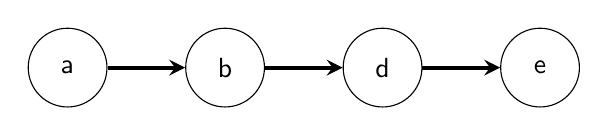
\begin{tikzpicture}[every node/.style={circle, draw, minimum size=10mm}]
            \node (a) at (0,0) {a};
            \node (b) at (2,0) {b};
            \node (d) at (4,0) {d};
            \node (e) at (6,0) {e};
        
            \draw[->, >=stealth, line width=1.5pt] (a) -- (b);
            \draw[->, >=stealth, line width=1.5pt] (b) -- (d);
            \draw[->, >=stealth, line width=1.5pt] (d) -- (e);
        \end{tikzpicture}
        \caption{Log of events on replica $x$}
        \label{fig:timewarp} 
    \end{subfigure}

    \vspace{5mm}

    \begin{subfigure}{1\linewidth}
        \centering
        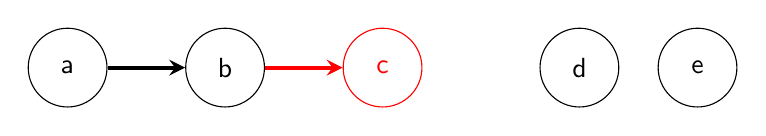
\begin{tikzpicture}[every node/.style={circle, draw, minimum size=10mm}]
            \node (a) at (0,0) {a};
            \node (b) at (2,0) {b};
            \node[red] (c) at (4,0) {c};
            \node (d) at (6.5,0) {d};
            \node (e) at (8,0) {e};
        
            \draw[->, >=stealth, line width=1.5pt] (a) -- (b);
            \draw[->, >=stealth, line width=1.5pt, red] (b) -- (c);
        \end{tikzpicture}
        \caption{Replica $x$ undoes updates $d$ and $c$ to apply out-of-order update $c$}
        \label{fig:timewarp}
    \end{subfigure}

    \vspace{5mm}

    \begin{subfigure}{1\linewidth}
        \centering
        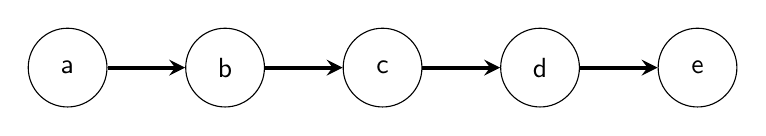
\begin{tikzpicture}[every node/.style={circle, draw, minimum size=10mm}]
            \node (a) at (0,0) {a};
            \node (b) at (2,0) {b};
            \node (c) at (4,0) {c};
            \node (d) at (6,0) {d};
            \node (e) at (8,0) {e};
        
            \draw[->, >=stealth, line width=1.5pt] (a) -- (b);
            \draw[->, >=stealth, line width=1.5pt] (b) -- (c);
            \draw[->, >=stealth, line width=1.5pt] (c) -- (d);
            \draw[->, >=stealth, line width=1.5pt] (d) -- (e);
        \end{tikzpicture}
        \caption{Replica $x$ reapplies updates $d$ and $c$ on top of $c$}
        \label{fig:timewarp}
    \end{subfigure}
    \caption{Demonstration of time warp progression}
    \label{fig:timewarpmain}
\end{figure}

This technique can be used to allow local-first collaboration with the help of a centralized server. Assume that the clients are able to perform time warp. The centralized server receives update messages from clients and writes them to an append-only log. Let clients adhere to the following algorithm when producing updates:

\begin{enumerate}
    \item Add an update to the local log
    \item Notify the server about the update
    \item Wait for the server to process the update
    \item Recieve response from the server that the update was successfully committed
    \item Mark the update as committed
\end{enumerate}

Alternatively if the client went out of sync:

\begin{enumerate}
    \item Add an update to the local log
    \item Notify the server about the update
    \item Wait for the server to process the update
    \item Recieve response from the server that the update is out of sync. The server also sends the updates that must be applied by this client to sync with the server.
    \item Client uses time warp to undo local updates and apply sync updates.
    \item If local updates produce no conflicts, they are applied again, otherwise the user can be prompted to resolve the conflicts. The original updates are discarded, and if the user resolves the conflict, new updates are generated.
\end{enumerate}

Notice that even if the update that the server received is out of sync, it can still be committed if it produces no conflicts. When the server sends the client a list of sync updates, it can also inform the client that the out of sync update was committed successfuly after the sync updates. Then the client can also apply this local update after applying all the sync updates - there is no need to discard it. TODO: MAYBE UNCLEAR, ADD PICTURE?

To employ this approach, it is crucial that the client is able to revert recent updates. Unfortunately, this functionality doesn't come built-in with most relational databases, including Postgres. To allow time warp on a database, one would have to be able to generate undo operations for all possible transactions. One notable challenge is recovering rows that where deleted as a side-effect of removing a foreign key they were referencing. Another challenge comes from the fact that transactions usually can't be organized into a strictly ordered sequence. In Postgres, multiple transaction isolation levels are supported, and only the strongest level, called SERIALIZABLE, has this property. See Serializable Isolation Level documentation \cite{tisolevel} for more details.

\subsection{Transaction replay approach}

The Colloboque server stores a history of committed Postgres database transactions and the state of the project after each transaction. When a client loses connection to the server, he keeps commiting transactions locally. When connection is re-established, the set of changes applied by the client is sent to the server. The server then takes the state of the project that the out-of-sync client based its changes on and uses it to start two transactions. The first transaction contains all the changes that the client applied locally, while the second transaction contains all the changes processed by the server while the client was disconnected. 

\subsubsection{Postgres transaction isolation levels} 
In the described approach transactions have to make use of isolation level REPEATABLE READ, which is stronger than the default transaction isolation level.

The default mode for transactions in Postgres is READ COMMITTED \cite{tisolevel}. It means that a transaction is allowed to read changes that where committed by other transactions after the current transaction has started. 

\begin{minted}[frame=single,linenos]{sql}
BEGIN;
SELECT * FROM data; -- 0 rows
-- another transaction commits inserting a row
SELECT * FROM data; -- 1 row
COMMIT;
\end{minted}

When using REPEATABLE READ transaction mode, the changes from newly committed transactions are not visible, but if the current transaction makes a conflicting update, it will lead to a serialization error.

\begin{minted}[frame=single,linenos]{sql}
BEGIN TRANSACTION ISOLATION LEVEL REPEATABLE READ;
SELECT * FROM data; -- 1 row
-- another transaction commits deleting a row
SELECT * FROM data; -- 1 row
UPDATE data SET col = 1;
-- ERROR:  could not serialize access due to concurrent delete
\end{minted}

With this approach the Postgres database can reliably identify whether the changes that the client made offline produce confilcts. If there are conflicts, the server discards the changes. The client will then have to sync with the server. An out-of-sync version of the document can be saved as a copy so that the user can compare the two versions manually.

\subsection{Data Branching}

Data branching in databases refers to the practice of creating divergent versions of data within a database, often for the purpose of testing, experimentation, or parallel development. This concept is similar to branching in version control systems like Git, but applied to data within a database rather than code in a repository.

Data branching could solve some problems posed by the Time Warp and Transaction replay approaches. In case of Time Warp, there is no need to undo operations if there exists a branch that contains the required version of the project. In case of Transaction replay, there would be no need to store the state of the project after each transaction. 

One example of data branching for Postgres is Neon \cite{neon}. Unfortunately, the free version of Neon only allows to create 10 branches, which is not enough for the purposes of GanttProject.

TODO: WRITE MORE?

\section{GanttProject}

GanttProject is an open-source desktop application for creating Gantt charts. A Gantt chart is a type of bar chart that illustrates a project schedule. It's a visual representation of the tasks and activities that need to be completed, along with their corresponding start and end dates. Gantt charts often include dependencies between tasks, showing which tasks must be completed before others can start. These dependencies are typically represented by arrows or lines connecting the bars. Some Gantt charts also include information about resource allocation, showing which resources (such as personnel or equipment) are assigned to each task.

GanttProject is written in Java and Kotlin and uses Postgres for the database. It supports saving projects in the cloud, but they can't be edited simultaneously by multiple people. GanttProject interface is shown on \Cref{fig:ganttscreen} 

\begin{figure}
    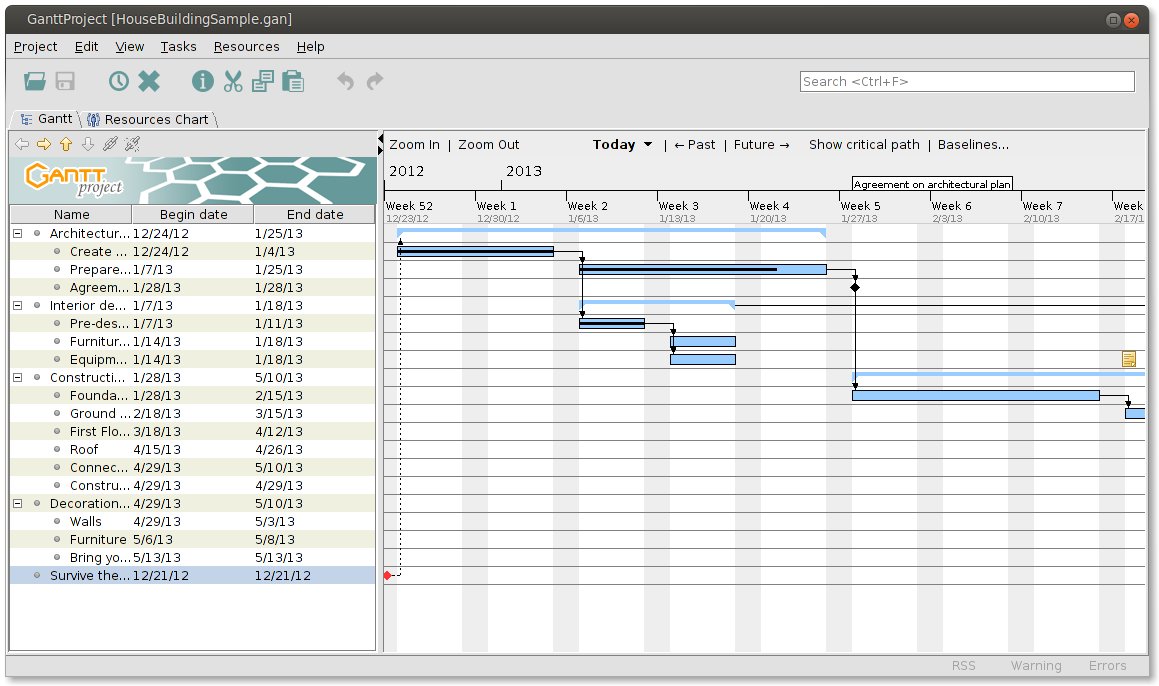
\includegraphics[width=\linewidth]{img/ganttproject.png}
    \caption{GanttProject interface}
    \label{fig:ganttscreen}
\end{figure}

\subsection{Colloboque}
To enable real-time collaboration in GanttProject, a module called Colloboque is being developed. It is written in Kotlin. Before I started working on Colloboque, it worked as follows.

Clients connect to a centralized Colloboque server and the server responds with an XML file describing the current version of the project. It was supposed to be the last version of the project, but the stub implementation responded with the same default project every time. The client recieved and loaded the project XML sent by the server. After that every change made by the user is wrapped into an update message and sent to the server. The client waits for the server to respond with a commit message. Until a response from the server is recieved, new changes are not allowed. 

% TODO: WHAT HAPPENS IF COMMIT FAILED?

The server recieves messages from clients. Each message contains information about a transaction that the client wants to perform. The server assigns a transaction id to each transaction, and the client's message includes the transaction id that the client last observed. If the server's last transaction id and the base transaction id in the update message do not match, the server informs the client about the error.

If the transaction ids match, the server executes the transaction, generates a commit message and propagates it to all connected clients.

This implementation had a few problems:

\begin{enumerate}
    \item Imagine a simple situation. A new project is created, let's denote the initial state of the project as $p$. Then one client connects and makes a change, producing a second version of the project - let's denote the second version $p'$. After that a second client connects to the same project. While it is expected that the server would share the latest version of the project $p'$ with the new client, this wasn't the case. In reality, the server would always respond to all newly connected clients with the same default project template $p$.
    \item The transactions performed by the server were not logged. This means that if a client was disconnected during some update, then this update is completely lost for this client. The server doesn't have the ability to generate an XML file describing the project from the database state, so recovery was not possible in this situation.
    \item When a client performs and update, he has to wait for confirmation from the server. During that time he can't introduce more updates. This makes collaboration in GanttProject not local-first. While it was never intended to be local-first in the first place, it is a nice feature that can be introduced.
\end{enumerate}

\subsection{Data model}
Due to the way relational databases work, conficts may arise in places where, intuitively, they shouldn't. For example, if one client tries to change task duration, while another tries to change task description, they will run into a conflict. This is because in the database all information about a task is stored in a single row. When clients try to concurrently change task duration and task description, they are essentially trying to change the same row. This will lead to an error if the two transactions happen to run in parallel on the server.

To avoid that, the data model on the Colloboque server differs from the one on the client. The client's \verb|Task| table can be found on \Cref{fig:client-database-init}. On the server this table is separated into multiple tables, each table containing \verb|uid| of the task and some of the attributes of the original \verb|Task| table, grouped either by logic or attribute type. A view object joins all the tables and provides an interface that allows to query all the different tables as if they where a single \verb|Task| table. Additionally, triggers are specified to handle updates and insertions called on the view, so that they are performed on the underlying tables. The server's \verb|Task| view definition can be found on \Cref{fig:server-database-init}

\begin{figure}
    \inputminted[frame=single,linenos]{sql}{lst/client-database-init.sql}
    \caption{Task table definition on a GanttProject client}
    \label{fig:client-database-init}
\end{figure}

\begin{figure}
    \inputminted[frame=single,linenos,fontsize=\small]{sql}{lst/server-database-init.sql}
    \caption{Task view definition on a GanttProject Colloboque server}
    \label{fig:server-database-init}
\end{figure}


\section{Implementation}

TODO: Implementation is a huge work in progress and the results are not very tangible as of now.

\subsection{jOOQ}

The first step in the implementation of local-first collaboration in GanttProject was to integrate jOOQ library \cite{jooq} with the existing server schema.

jOOQ can generate Java classes based on the database schema, describing tables, columns, and so on. These generated classes provide type-safe access to the database objects, eliminating the need for manual SQL string concatenation and reducing the risk of SQL injection attacks. jOOQ also abstracts away the differences between SQL dialects. This allows to write database-agnostic code that can be easily ported.

TODO: DESCRIBE THIS PARAGRAPH MORE FORMALLY OR EDIT OUT. There were some problems due to jOOQ being bugged. Enum classes where not visible outside of a schema and enum class names had to be written in a specific way for them to be recognized at the class generation step. For example \verb|TaskIntPropertyName| had to be written as \verb|"taskintpropertyname"| in the actual script (\Cref{fig:server-database-init}, line 12).

\subsection{Restoring the latest version}

The next step was to make the server return the latest version of the project to newly connected clients.

To do that the server first had to persist transaction log. This would allow the server to calculate the relevant version of the project by taking the initial XML project file and repeatedly applying transactions to it.

The source code of the client contains logic for loading project from XML into an in-memory H2 database. This logic was exposed in Colloboque. When a new client connected, the server would load the XML project template into an in-memory database, apply transactions from the transaction log table to it, save the resulting project as an XML and send it to the client. 

This way new clients would recieve a relevant version of the project, not a project template, as it was before. 

\subsection{Transaction replay}

The last step is to implement transaction replay approach and enable local-first collaboration.

I've implemented a function, which takes a database and two sets of update logs. It creates two connections and starts a transaction on each of the connections. Both transactions run with isolation level REPEATABLE READ. After starting the transactions, the function applies one set of updates in one transaction, and the second set of updates in another transaction.  Finally it tries to commit both transactions, and either returns true if both commits where successful, or false if there was an error.

Unfortunately, the execution never manages to reach the commit stage. When the second set of updates is being applied, the code hangs indefinitely. It seems that there is some kind of a deadlock in the database. Changing transaction isolation level to READ COMMITTED doesn't affect this behavior. This problem needs further investigation. See function code on \Cref{fig:merge-fun}

\begin{figure}
    \inputminted[frame=single,linenos,breaklines]{kotlin}{lst/merge-concurrent-updates.kt}
    \caption{Function for trying transaction replay}
    \label{fig:merge-fun}
\end{figure}

\subsection{Protocol}

\subsubsection{Outline}

The client can generate local updates and accept updates from the server. Local and server updates are processed synchronously by the client. Local updates are communicated to the server after the client applies them. The server processes all client updates synchronously and establishes a total order of the events by assigning incrementing ids. The client has to follow the total order of the events established by the server. The client can deviate from the established order because it applies local updates without getting confirmation from the server. Upon discovering errors in the order of applied events, the client enters synchronization phase. In synchronization phase the client stops accepting updates. It takes all local updates that are not confirmed by the server yet, and sends them to the server. The server uses Transaction Replay approach (TODO: CITE THE CORRESPONDING SECTION) to check whether the updates produce conflicts. If they don't produce conflicts, the server applies them. Finally, the server responds to the client with the latest state of the project and an indication whether the client's updates were applied or not.

\subsubsection{Server}




\newpage
\printbibliography
\clearpage
\end{document}